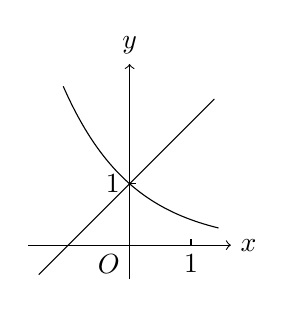
\begin{tikzpicture}[x=.78cm,y=.78cm,baseline=(current bounding box.center)]
  \draw[->] (-1.65,0)--(1.65,0) node[right] {$x$};
  \draw[->] (0,-.55)--(0,2.95) node[above] {$y$};
  \draw[domain=-1.08:1.45,samples=100,smooth] plot (\x,{exp(-.88*\x)});
  \draw (-1.48,-.48)--(1.38,2.38);
  \draw (1,0)--(1,.10) (0,1)--(.10,1);
  \node[below] at (1,0) {$1$}; \node[left] at (0,1) {$1$}; \node[below left] at (0,0) {$O$};
\end{tikzpicture}
